\providecommand{\paper}[1]{#1}
\providecommand{\thesis}[1]{}

\paper{
\newcommand{\pth}{.}
\newcommand{\this}{paper}
\documentclass{article}
\usepackage{amssymb, amsthm, graphicx, float, textcomp, bnaic}
\title{\textbf{\Huge Visualisation on a Closed Surface}}
\author{Walter A. Kosters and Jeroen F. J. Laros}
\date{\textit{Leiden Institute of Advanced Computer Science (LIACS)}\\
      \textit{Universiteit Leiden, The Netherlands}\\
      \texttt{jlaros@liacs.nl}}
\frenchspacing
\setlength{\parindent}{0pt}

\newtheorem{theorem}{Theorem}
\newtheorem{lemma}[theorem]{Lemma}
\newtheorem{corollary}[theorem]{Corollary}

\theoremstyle{definition}
\newtheorem{example}[theorem]{Example}
\newtheorem{definition}[]{Definition}
\newtheorem{remark}[theorem]{Remark}
\newtheorem{conjecture}[theorem]{Conjecture}

\pagestyle{empty}

\begin{document}
\ttl
\thispagestyle{empty}

%\maketitle
}

\paper{\begin{abstract} \noindent  We propose}\thesis{In this \this, we
discuss} a visualisation algorithm that, given a set of points in
high-dimensional space, will produce an image projected on a 2-dimensional
torus. The algorithm is a push and pull oriented technique which uses a
sigmoid-like function to correct the pairwise distances. We describe how to
make use of the torus property and show that using a torus is a generalization
of employing the standard closed unit square. Experiments show the merits of
the method.
\paper{
\end{abstract}
}

\section{Introduction}\label{to:introduction}
In many situations one wants to cluster and/or visualise data~\cite{TSK}. In
this \this\ we will describe a method to visualise a perhaps large set of data
points on a 2-dimensional surface. This surface is basically the unit square
$U$ in $\mathbb{R}^2$, with sides identified in such a way that it
topologically is a \emph{torus}: left and right boundary are identified, and so
are top and bottom boundary, see Figure~\ref{to:thesquare} below. The resulting
surface has no boundaries. As distance between two points $a$ and $b$ in $U$
we just take the minimum of the ordinary Euclidean distance between $a$ and any
point from $\{b+(k,\ell)\;|\;k,\ell\in\{-1,0,1\}\}$. This surface will be
referred to as ``the'' torus. Note that the distance is \emph{not} the one
that arises when a torus is embedded in $\mathbb{R}^3$ in the usual way (as a
doughnut). In our case a visualisation as a unit square is more appropriate,
remembering that left-hand and right-hand side are near to one another (and
also top side and bottom side).


\begin{figure}[!ht]
\begin{center}
\begin{picture}(100,60)(-20,0)
\thicklines
\put(40,0){\vector(1,0){10}}
\put(0,0){\line(1,0){7}}
\put(10,0){\line(1,0){7}}
\put(20,0){\line(1,0){7}}
\put(30,0){\line(1,0){7}}
\put(0,0){\vector(0,1){50}}
\put(40,50){\vector(1,0){10}}
\put(0,50){\line(1,0){7}}
\put(10,50){\line(1,0){7}}
\put(20,50){\line(1,0){7}}
\put(30,50){\line(1,0){7}}
\put(50,0){\vector(0,1){50}}
\put(-15,0){\makebox(0,0){$(0,0)$}}
\put(-15,50){\makebox(0,0){$(0,1)$}}
\put(65,0){\makebox(0,0){$(1,0)$}}
\put(65,50){\makebox(0,0){$(1,1)$}}
\put(35,15){\makebox(0,0){$U$}}

\end{picture}
\end{center}
\caption{Unit square with sides identified: the torus.}\label{to:thesquare}
\end{figure}


\paper{So we}\thesis{We} start with a finite set of $n$ data points
$\{p_1,p_2,\ldots,p_n\}$. We use \paper{some}\thesis{a} given metric $d$ to
compute the distance $d_{ij}=d(p_i,p_j)$ between $p_i$ and $p_j$
($i,j\in\{1,2,\ldots,n\}$), which yields a symmetric matrix
$D=(d_{ij})_{i,j=1}^n$. This matrix $D$ will be the basis for our further
actions. Its entries will be referred to as the \emph{desired distances}. Our
goal is to obtain points $\{p_1',p_2',\ldots,p_n'\}$ (the so-called
\emph{current points}) in $U$, in such a way that the distance between $p_i'$
and $p_j'$ in $U$ (the \emph{current distance}) resembles $d_{ij}$, the desired
distance between $p_i$ and $p_j$, as much as possible for
$i,j\in\{1,2,\ldots,n\}$. The difference between the current distances and the
desired distance is therefore minimised. Together, the current points
constitute the \emph{current configuration}. Once this configuration is
established, it can be used for all sorts of clustering purposes.

Our algorithm repeatedly takes two current points, and pushes them together or
pulls them apart with a \emph{correction factor}, depending on the relation
between desired and current distance. We use an \emph{inflation factor} and a
\emph{correction multiplier} to improve the current configuration. Note that
the distances in $U$ do not change when one rotates, mirrors or translates all
points. Since our method makes use of random elements, visualisations might be
the same under rotation, mirroring or translation, but it is also possible
that they are actually different.

There are many methods that perform a dimension reduction. We mention Multi
Dimensional Scaling (MDS, see~\cite{BG,HTF}) and Principal Component Analysis
(PCA, see~\cite{HTF}) as two well-known statistical methods. Other methods
include several types of (competitive) neural networks, such as Kohonen's Self
Organizing Maps (SOMs, see~\cite{HTF})
and vector quantization (again, see~\cite{HTF}). A comparison of all these methods is
beyond the scope of this \this\ (e.g., see~\cite{F}), we just mention two
issues. First, our method is intuitive, very fast and requires no complicated
mathematical operations, such as matrix inversion. Second, the use of the
torus appears to be both natural and easy to describe; it also performs better
than the previously used closed unit square (with boundary, cf.~\cite{KW}), but
still has all its merits. Notice that when using a $0.5\times0.5$ sub-square of
$U$, one has this situation as a special case.

In Section~\ref{to:space} we sketch the background, and mention some alternative
topologies. The method is described in Section~\ref{to:alg}. Section~\ref{to:exps}
has experiments, and we conclude in Section~\ref{to:conclusion}.


\section{Background}\label{to:space}
In this section we mention some issues concerning our
\paper{surface}\thesis{method}. We will also point out a few difficulties that
might arise, and some other possibilities.

As specified above, the surface we use is not the standard 2-dimensional unit
square in the Euclidean space $\mathbb{R}^2$, but a 2-dimensional torus. The
main advantage of using such a manifold is that there are more degrees of
freedom in such a space.

A disadvantage of using a torus is that it is impossible to contract every
circle to a point, and thus there are configurations possible where clusters
are wrapped around the torus and thus might get stuck in a ``local minimum''.
A solution to this is to use a sphere (where each circle can be contracted to a
point), but the projection of a globe onto a flat 2-dimensional space gives a
distorted image (just like the map of the earth, the polar regions usually
appear much larger than they actually are).

Another way to prevent the potential wrapping around the torus is to use a
non-random initialization. If all points are initialized in one (small) area,
the process will most likely not result in a configuration where wrapping is
an issue. This can even be forced by placing a maximum distance (determined by
the circumference of the torus) on the correction part of the algorithm.

There are more possibilities for such surfaces, like the non-orientable Klein
bottle (obtained when identifying the dotted arrows from
Figure~\ref{to:thesquare} in opposite direction) or the real projective plane, but from all these, the metric on a torus
(as specified above) is most like the standard Euclidean one, so it is natural
to choose this object.

\section{Algorithm}\label{to:alg}
The algorithm we use is a \emph{push and pull} oriented one, where the
correction factor depends on the difference between the desired distance
$d_\mathrm{desired}$ and the current distance $d_\mathrm{current}$. This
current distance, or rather its square, between two points $a=(x_1, y_1)$ and
$b=(x_2, y_2)$ from $U$ can be efficiently computed by:
\vbox{
\vspace*{5mm}\hrule\vspace*{-1mm}
\begin{tabbing}
\paper{XXXXXXX}XXXXXXXX\=XXX\=Xy\=Xy\=Xy\=Xy\=XXXXXXXX\=XXXXX\=XX \kill
\>$d_\mathrm{current}\,((x_1, y_1),(x_2, y_2)) ::$\\
\>\>$\mathbf{var\ } x_3 \leftarrow x_2;$\\
\>\>$\mathbf{var\ } y_3 \leftarrow y_2;$\\
\>\>$\mathbf{if\ }\,x_1 - x_2 > 0.5 \mathbf{\ \ then\ }$ $x_3 \leftarrow x_3 + 1.0;$\\
\>\>$\mathbf{if\ }\,x_1 - x_2 < -0.5 \mathbf{\ \ then\ }$ $x_3 \leftarrow x_3 - 1.0;$\\
\>\>$\mathbf{if\ }\,y_1 - y_2 > 0.5 \mathbf{\ \ then\ }$ $y_3 \leftarrow y_3 + 1.0;$\\
\>\>$\mathbf{if\ }\,y_1 - y_2 < -0.5 \mathbf{\ \ then\ }$ $y_3 \leftarrow y_3 - 1.0;$\\
\>\>$\mathbf{return\ \ } (x_1 - x_3)^2 + (y_1 - y_3)^2\;;$
\end{tabbing}
\vspace*{-1mm}\hrule\vspace*{1mm}
\centerline{{Quadratic distance between points in $U$}}
\vspace*{1.2mm}
\hrule\vspace*{5mm}
}
\noindent
The point $b'=(x_3,y_3)$ is the (or more precisely, a) point from
$\{b+(k,\ell)\;|\;k,\ell\in\{-1,0,1\}\}$ that realizes the shortest distance to
$a$. This point will also be used later on. The maximal quadratic distance
between any two points from $U$ equals $0.5$. (We will omit the word
``quadratic'' in the sequel.)

Instead of a linear or a constant function (of the current distance) to
calculate the amount of correction, we can and will use a sigmoid-like
function, or rather a family of functions. This function must adhere to some
simple constraints, enumerated below. So we want a function
$f=f_{d_\mathrm{desired}}$ which is defined on $[0,0.5]$, where $0.5$ is the
maximum distance between two points (on the torus). We must have, with
$0<d_\mathrm{desired}<0.5$ fixed:
\begin{itemize}
\item $f(0) = \rho$
\item $f(0.5) = -\rho$
\item $f(d_\mathrm{desired}) = 0$
\end{itemize}
Here $\rho\in(0,1]$ is the so-called \emph{correction multiplier}. So when the
current distance is as desired, $f$ has value 0 --- and so has the correction.
The resulting correction factor $\mathit{corrfac}$ equals
$f(d_\mathrm{current})$. If $d_\mathrm{desired}=0$, we make it slightly
larger; similarly, if $d_\mathrm{desired}=0.5$, we make it slightly smaller.

We will use
\begin{displaymath}
  f_{d_{\mathrm{desired}}}(x)=
  \left\{\begin{array}{ll}
  \rho\;\cos\;(\pi \log_t (2x (t - 1) + 1)) &\mathrm{\ if\ \;} d_\mathrm{desired} \neq 0.25 \\
  \rho\;\cos\;(\pi 2x) &\mathrm{\ if\ \;} d_\mathrm{desired} = 0.25
  \end{array}\right.
\end{displaymath}
where $t = (1-1/{(2d_\mathrm{desired})})^2$; this function satisfies all the
constraints. Figure~\ref{to:sinus} depicts $f_{0.1}$ and $f_{0.25}$, with $\rho=1$.

The reason we choose a function like this, is because the correction of a 
point will be large when the error of that point is large. Only when the 
error is close to zero, the correction will be small. Other functions, like
sigmoids will have the same behaviour. 

\begin{figure}[!ht]
\begin{center}
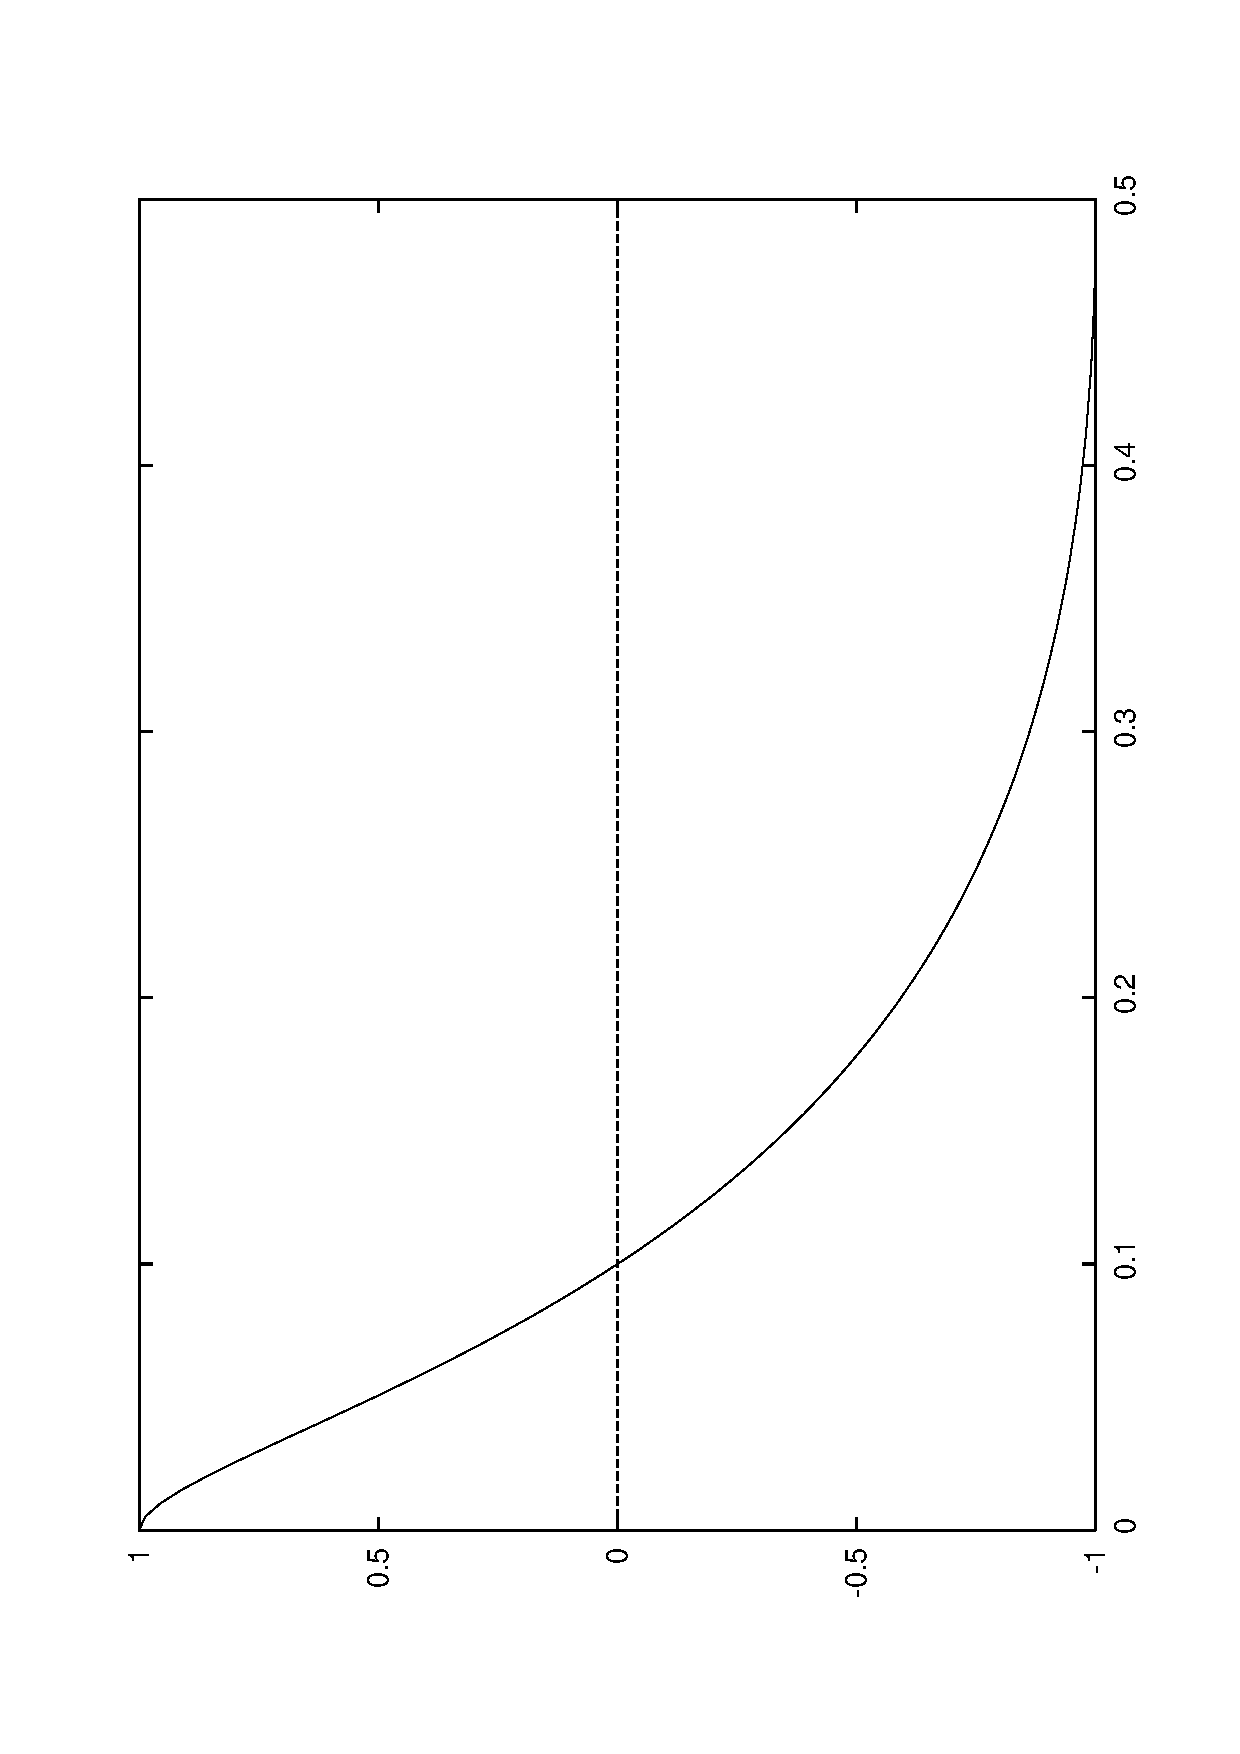
\includegraphics[angle=270, width=0.48\linewidth]{\pth/func}
\ 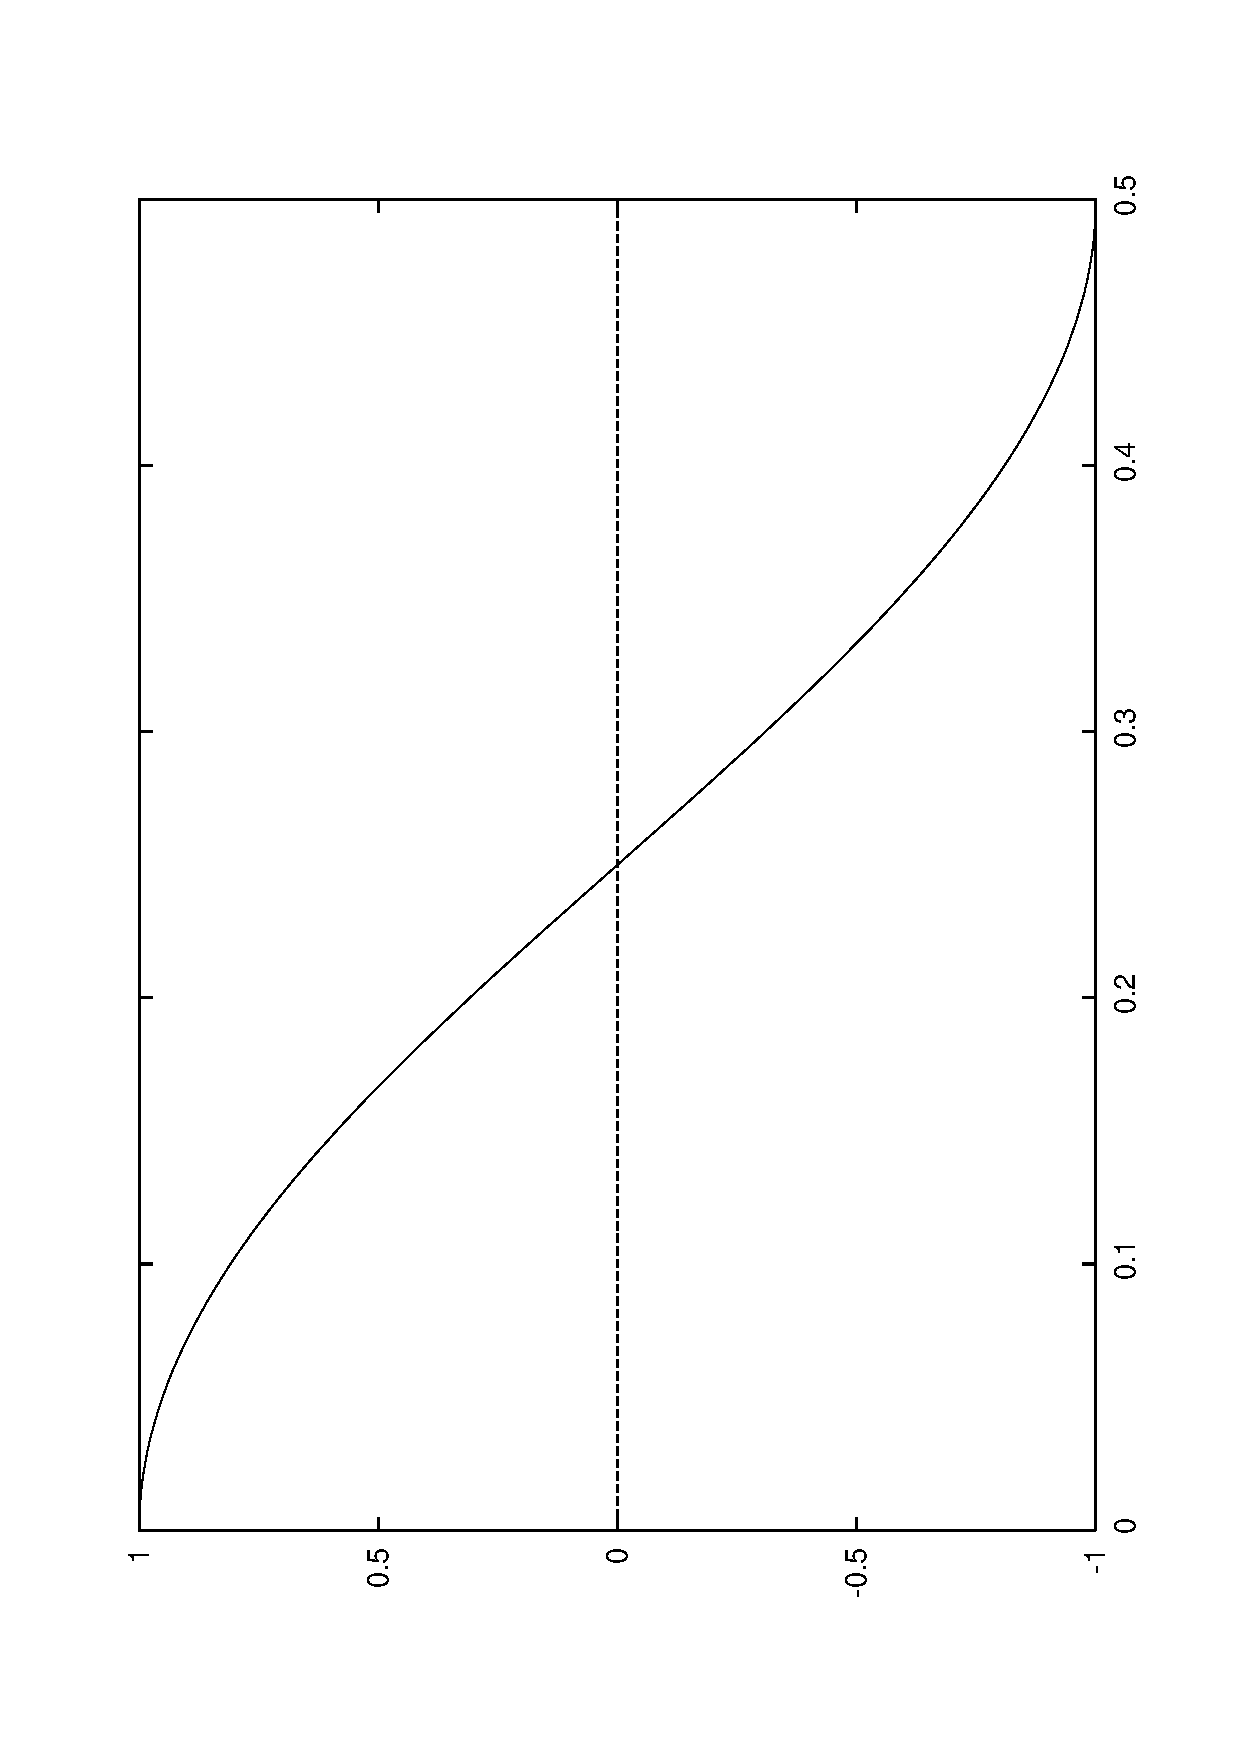
\includegraphics[angle=270, width=0.48\linewidth]{\pth/func0}
\caption{$f_{d_{\mathrm{desired}}}$ with $d_\mathrm{desired}=0.1$ and $d_\mathrm{desired}=0.25$, $\rho=1$.}\label{to:sinus}
\end{center}
\end{figure}

Now suppose we want to ``push and pull'' two given points $a=(x_1,y_1)$ and
$b=(x_2,y_2)$ in $U$; we first compute $b'=(x_3,y_3)$ as in the distance
calculation of $d_\mathrm{current}$ above. Then the coordinates $x_1$ and $y_1$ of
$a$ are updated through
\begin{eqnarray}
x_1 &\leftarrow& x_1 + \mathit{corrfac}\cdot|d_\mathrm{desired}-d_\mathrm{current}|\cdot(x_1-x_3)\;/\;2
\label{to:update}\\
y_1 &\leftarrow& y_1 + \mathit{corrfac}\cdot|d_\mathrm{desired}-d_\mathrm{current}|\cdot(y_1-y_3)\;/\;2
\nonumber
\end{eqnarray}
A positive $\mathit{corrfac}$ corresponds with pushing apart,
a negative one with pulling together.
In a similar way, the coordinates $x_3$ and $y_3$ of $b$ are updated in
parallel. If a coordinate becomes smaller than 0, we add 1, and if it becomes
larger than 1, we subtract 1. Together we will refer to this as
Equation~(\ref{to:update}).

The basic structure of the algorithm is as follows:

\vbox{
\vspace*{5mm}\hrule\vspace*{-1mm}
\begin{tabbing}
\paper{XXXXXXXXXX}XXXXX\=XXX\=Xy\=Xy\=Xy\=Xy\=XXXXXXXX\=XXXXX\=XX \kill
\>initialize all current points in a small region of $U$\\
\>$\mathbf{while\ not\ } \mathit{Ready} \mathbf{\ do}$ \\
\>\>update all pairs (in arbitrary order) with Equation (\ref{to:update})
\end{tabbing}
\vspace*{-1mm}\hrule\vspace*{1mm}
\centerline{{The push and pull algorithm}}
\vspace*{1.2mm}
\hrule\vspace*{5mm}
}
\noindent
The algorithm terminates when the standard deviation and the 
mean error 
($\sum_{|\mathrm{pairs}|}|d_{\mathrm{desired}} - d{\mathrm{current}}|/
|\mathrm{pairs}|$) no longer change.

We now introduce the inflation factor $\sigma$, and secondly comment on the
correction multiplier $\rho$.

\paper{
\subsection{Inflation factor}
}
The \emph{inflation factor} $\sigma>0$ can be used in the following way:
Equation~(\ref{to:update}) is changed to
\begin{eqnarray}
x_1 \leftarrow x_1 + \mathit{corrfac}\cdot|\sigma\cdot d_\mathrm{desired}-d_\mathrm{current}|\cdot(x_1-x_3)\;/\;2.
\label{to:update2}
\end{eqnarray}

This can be useful in several ways. If, for example, all distances are between
$0$ and $0.2$, one might argue that it is useful to multiply these distances by
$2.5$ to get a better spreading. This argument is especially valid if the
resulting clustering cannot be realized in the plane, but can be embedded on a
torus. Inflation with the right factor can make the overall error drop to zero
in this case, while using the original distances will always result in a
non-zero overall error.

Even if all distances are between $0$ and $0.5$, inflation or deflation can
still be beneficial. For example, the input data can be such that inflation or
deflation will result in the correct clustering of a large part of the input,
while not using an inflation factor will result in a much higher overall error.
An example of such input data would be a torus that is scaled between $0$ and
$0.2$, with a few points outside this region. Normal clustering would result in
a flat image where the points outside the torus region would have correct
distances to the torus region, but with the correct inflation factor, the torus
will be mapped on the entire space, and the few points outside the region will
be misclustered. This results in a clustering where the overall error is small.

In practice we often take $\sigma=1$.

\paper{
\subsection{Correction multiplier}
}
The correction multiplier $\rho$ is a parameter which controls the
aggressiveness of the correction function. Initially this factor is set to 1,
but for data that can not be embedded in the plane, lowering this factor can be
beneficial.

If, for example, most of the distances are near the maximum, the correction
function will push them so far apart, that they are pushed towards other points
at he other side of the torus. This can result in the rapid fluctuation between
two or more stable states. These states are probably not the global minimum for
the clustering error, and therefore not the end result we desire. Increasing
the correction multiplier will counter this effect.


\section{Experiments}\label{to:exps}
In this section we describe several experiments, both on synthetic and real
data. The experiments are of an exploratory nature. We try to give a good
impression of the merits of the algorithm.

We start with a synthetic dataset. In the left-hand picture of
Figure~\ref{to:fig:flat} we see the original data points (on a ``flat'' 2D plane),
from which a distance matrix is derived to serve as test data for the
visualisation algorithm. In this picture we see seven spheres of which three
are unique: the topmost two and the one in the center. The other four spheres
are copies of one another.  The total number of points is $700$ and all
distances are between $0.0$ and $0.5$.

\begin{figure}[!ht]
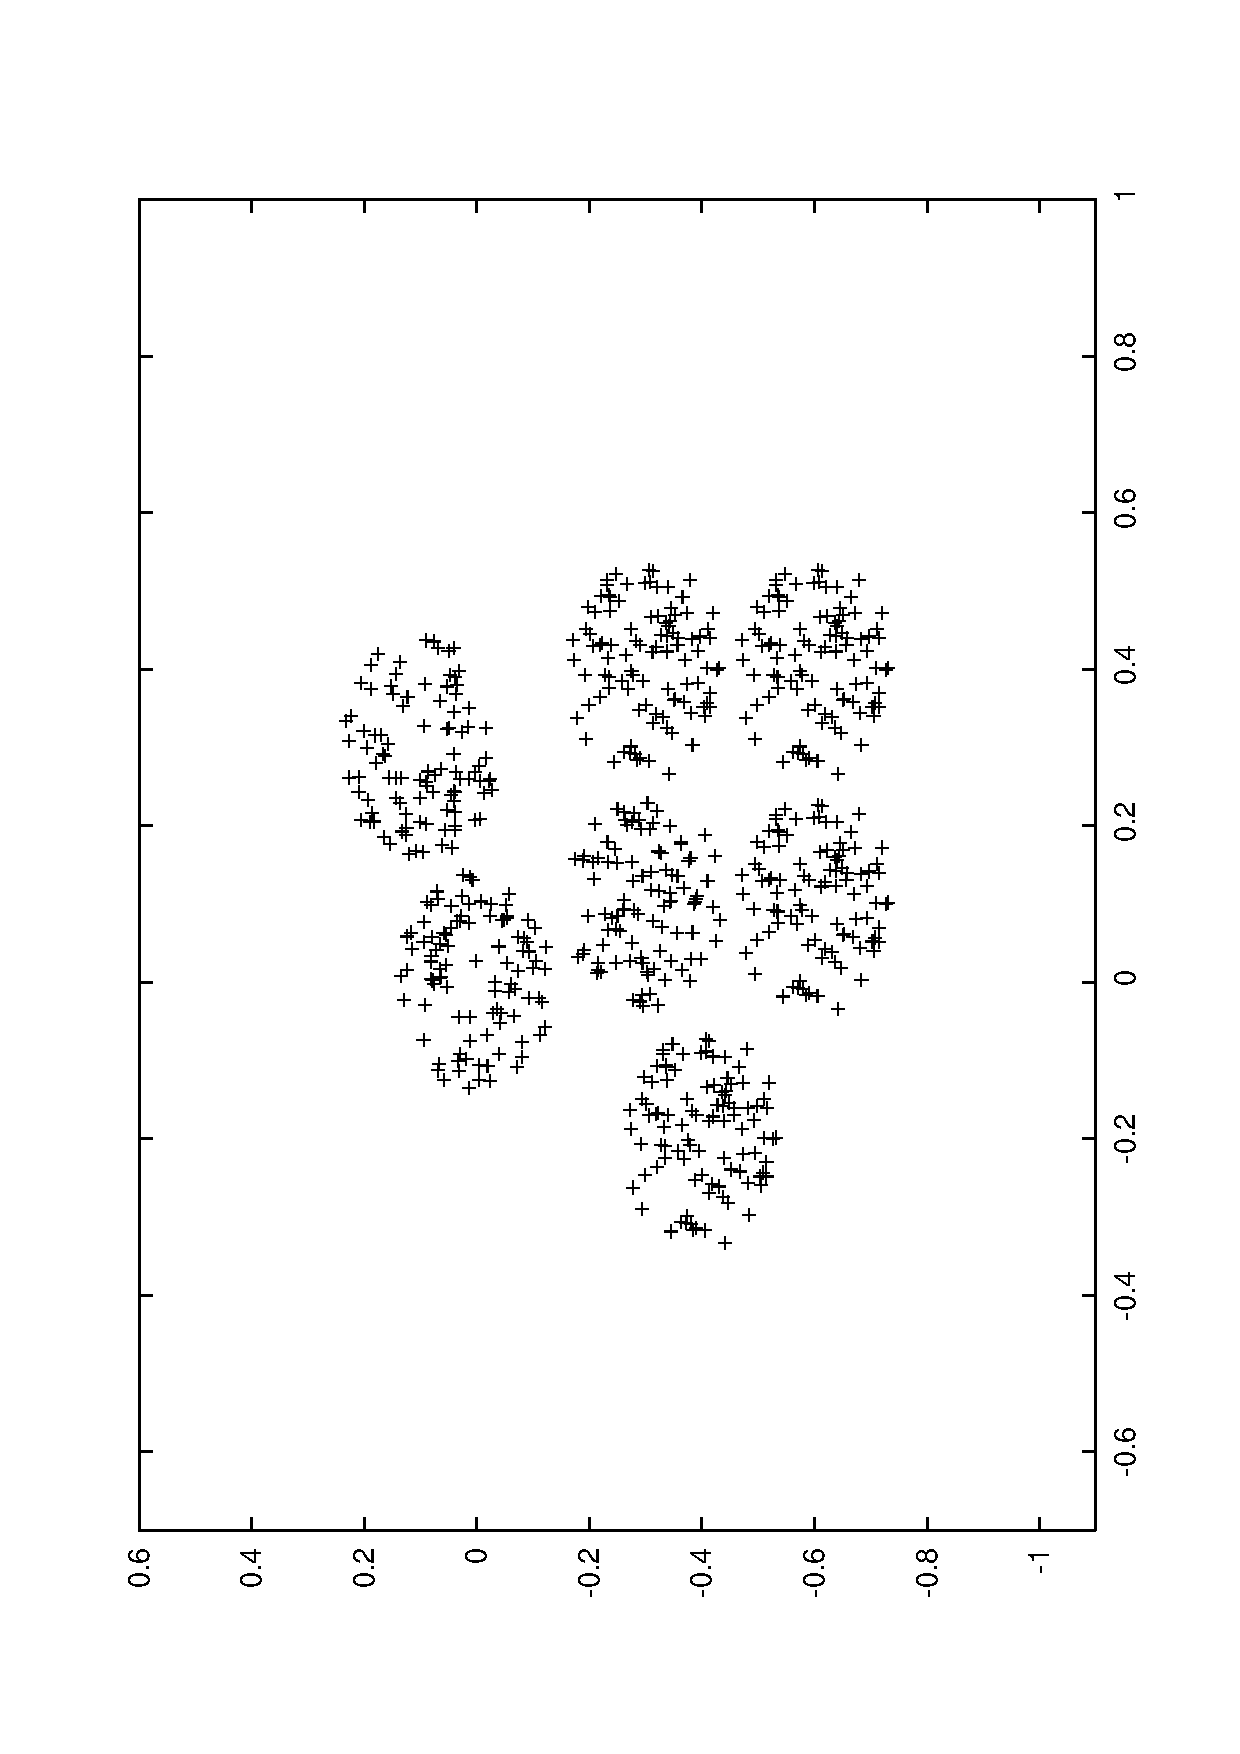
\includegraphics[angle=270, width=0.48\linewidth]{\pth/in}
\ 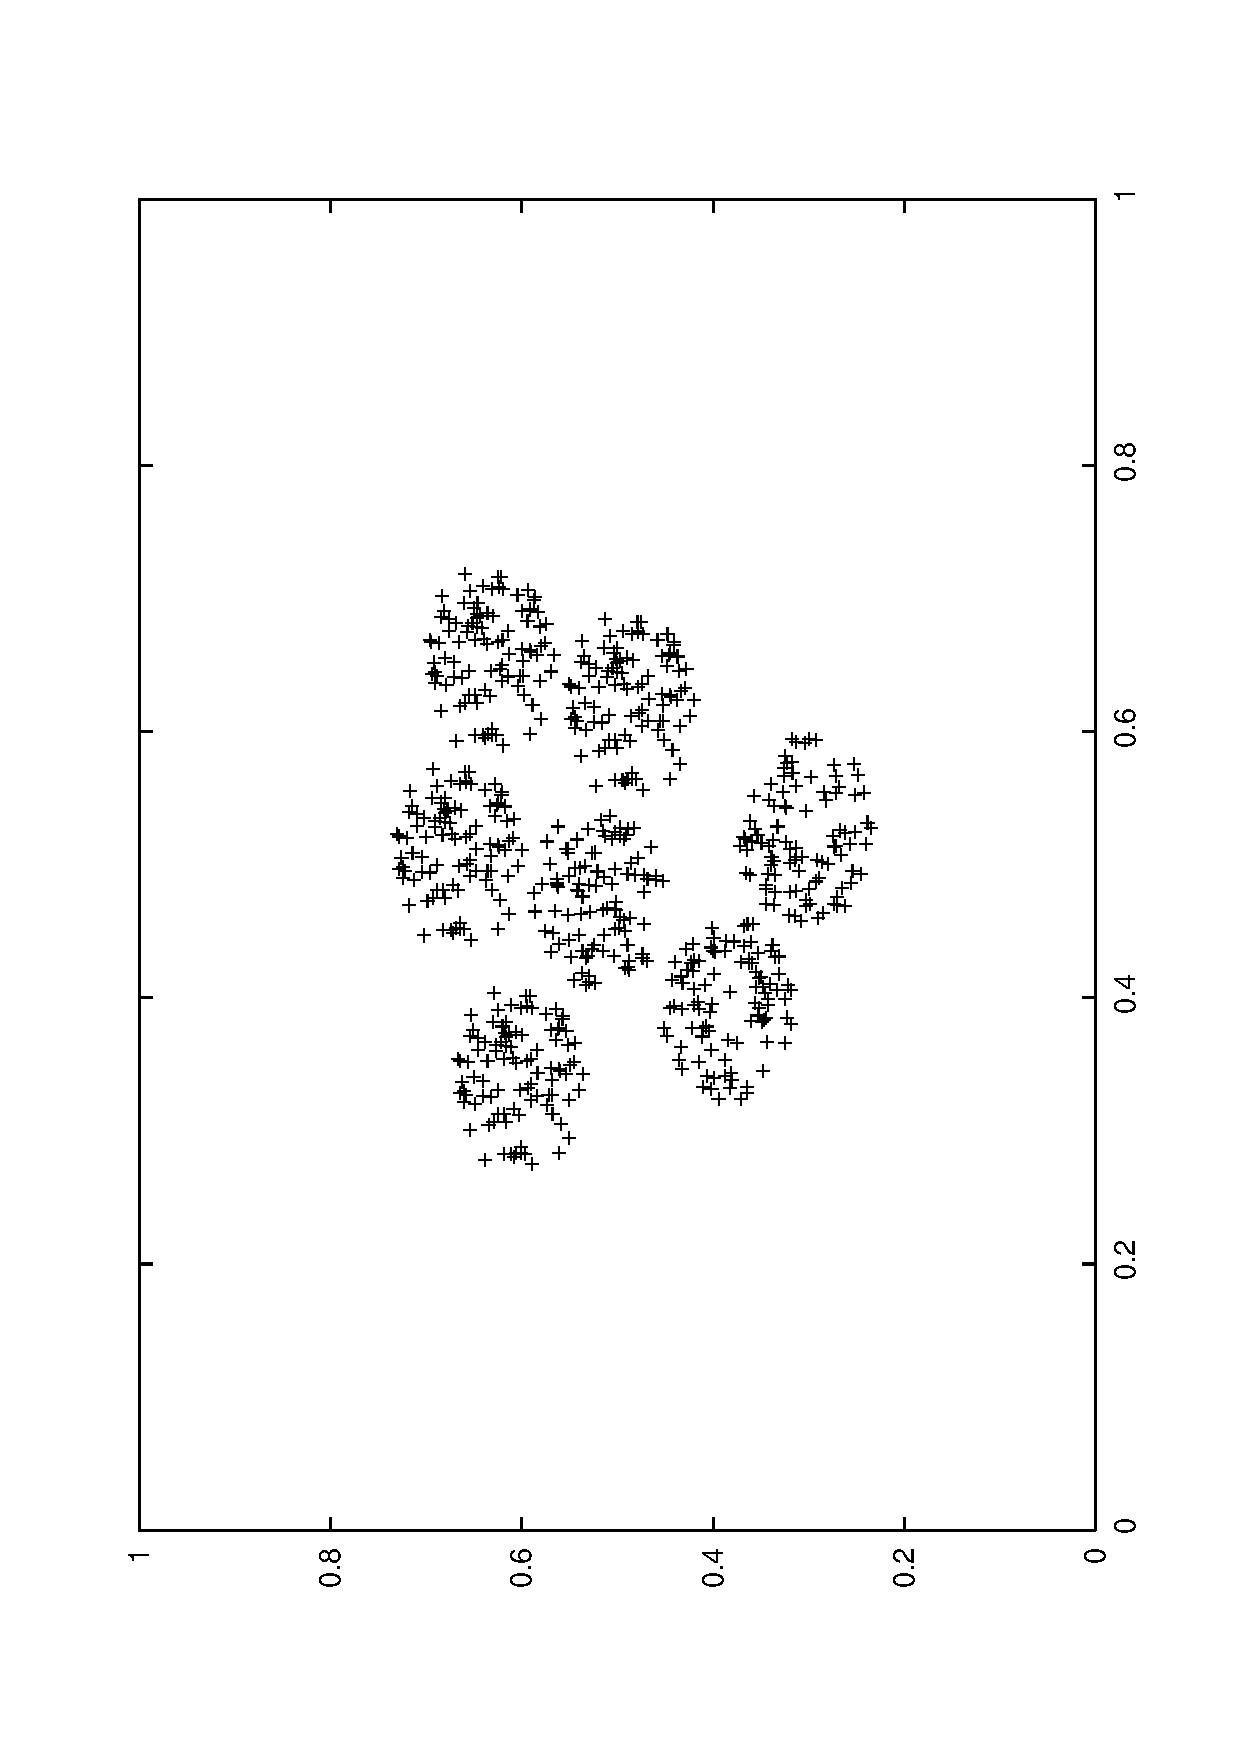
\includegraphics[angle=270, width=0.48\linewidth]{\pth/flat1}
\caption{Original data (left) and visualisation (right).} \label{to:fig:flat}
\end{figure}

After only a few iterations of our algorithm, the right-hand picture of
Figure~\ref{to:fig:flat} appears. Notice how it resembles the input data, except
for a mirroring and a rotation. All distances are preserved almost perfectly.
Remember that only the pairwise distances were used by the algorithm. The mean
error in this picture is $0.00004$ and the standard deviation is $0.00003$. As
a final remark, ``flat data'' will always cluster within a sub-square of size
$0.5 \times 0.5$.

\begin{figure}[H]
\begin{center}
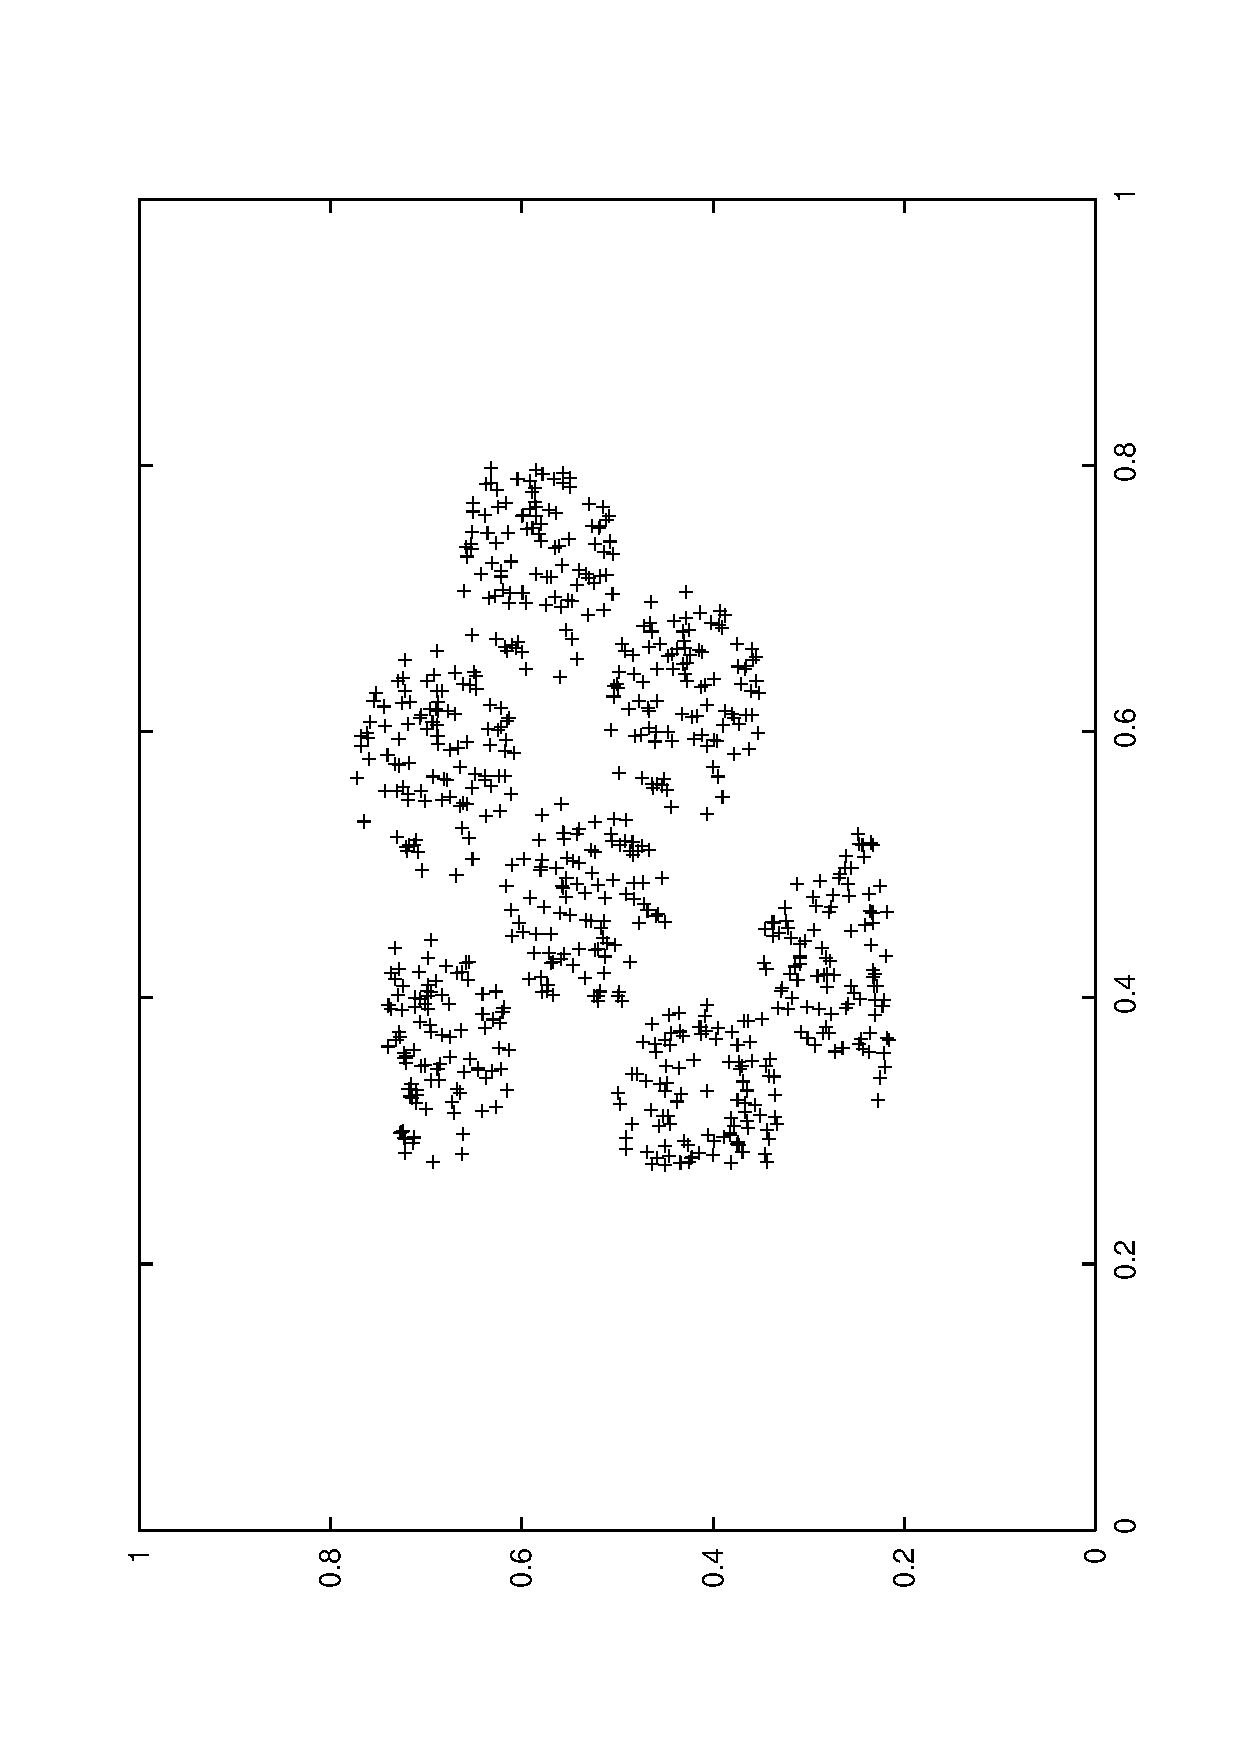
\includegraphics[angle=270, width=0.48\textwidth]{\pth/flat2}
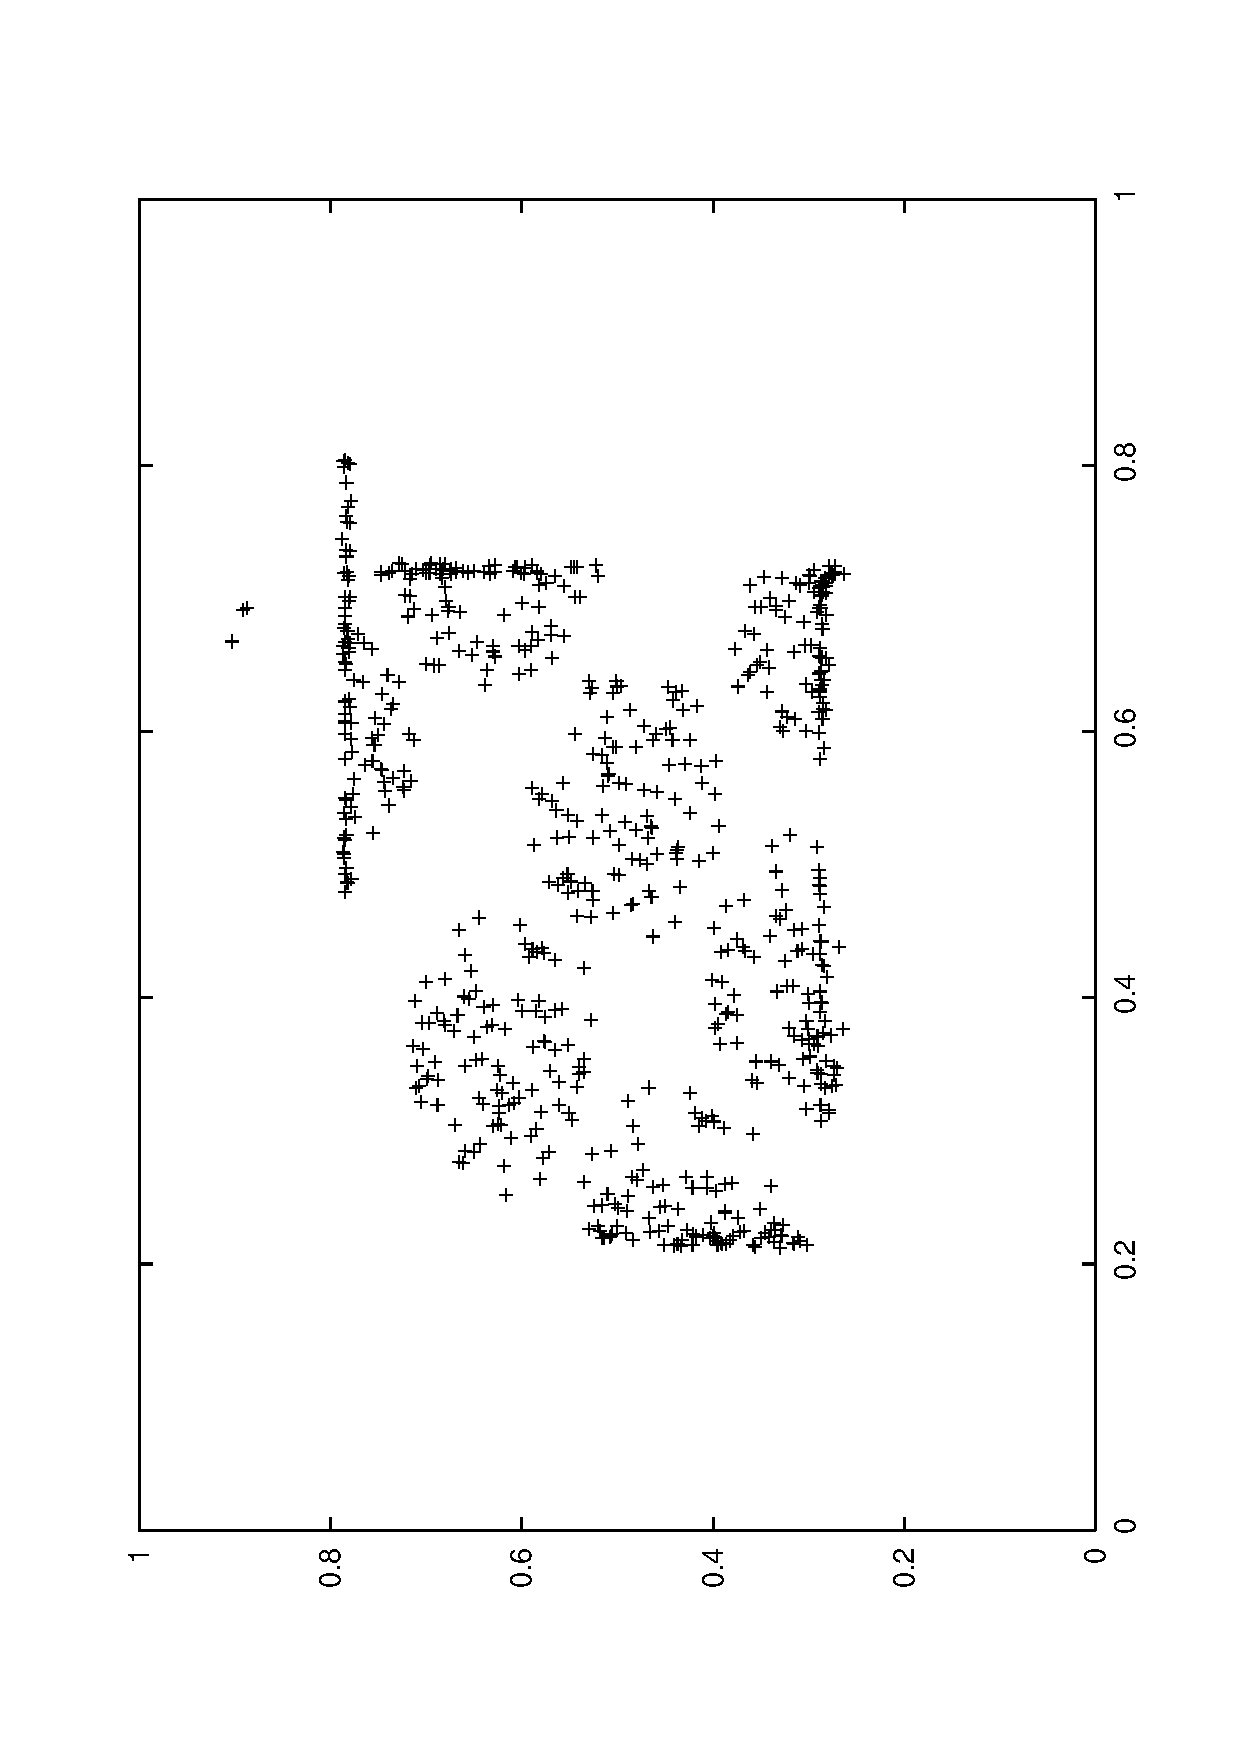
\includegraphics[angle=270, width=0.48\textwidth]{\pth/flat3}
\caption{Visualisation of flat data with an invalid inflation factor.}
\end{center}
\label{to:fig:clusinv}
\end{figure}
In Figure~\ref{to:fig:clusinv} we see the same test data, except that the
distances have been multiplied by a factor $1.5$ in the left-hand picture, and
by $2.6$ in the right-hand one. This results in a non-correct embedding, since
the maximum distance in this space is $0.5$. The effects can be seen in
Figure~\ref{to:fig:clusinv}, in particular in the right-hand picture. In both
pictures a translation has been applied in order to center most points. Though
the full $1.0\times 1.0$ square has been used, most current points reside in
the smaller $0.5\times 0.5$ square, as is clearly visible in the right-hand
picture.

The top-left sphere is forced closer to the bottom-left one than is possible.
This results in the flattening of the spheres at the outermost edges. This
effect can be explained by considering the overall error (which is minimized).
By a local deformation, the overall error is kept small. The effect can also
be seen (to a lesser extent) in the middle-left sphere. Notice that the effect
is absent in the top-central sphere because of the void at the bottom-center of
the picture (there is nothing to collide with at the other side of the torus).

\begin{figure}[!ht]
\begin{center}
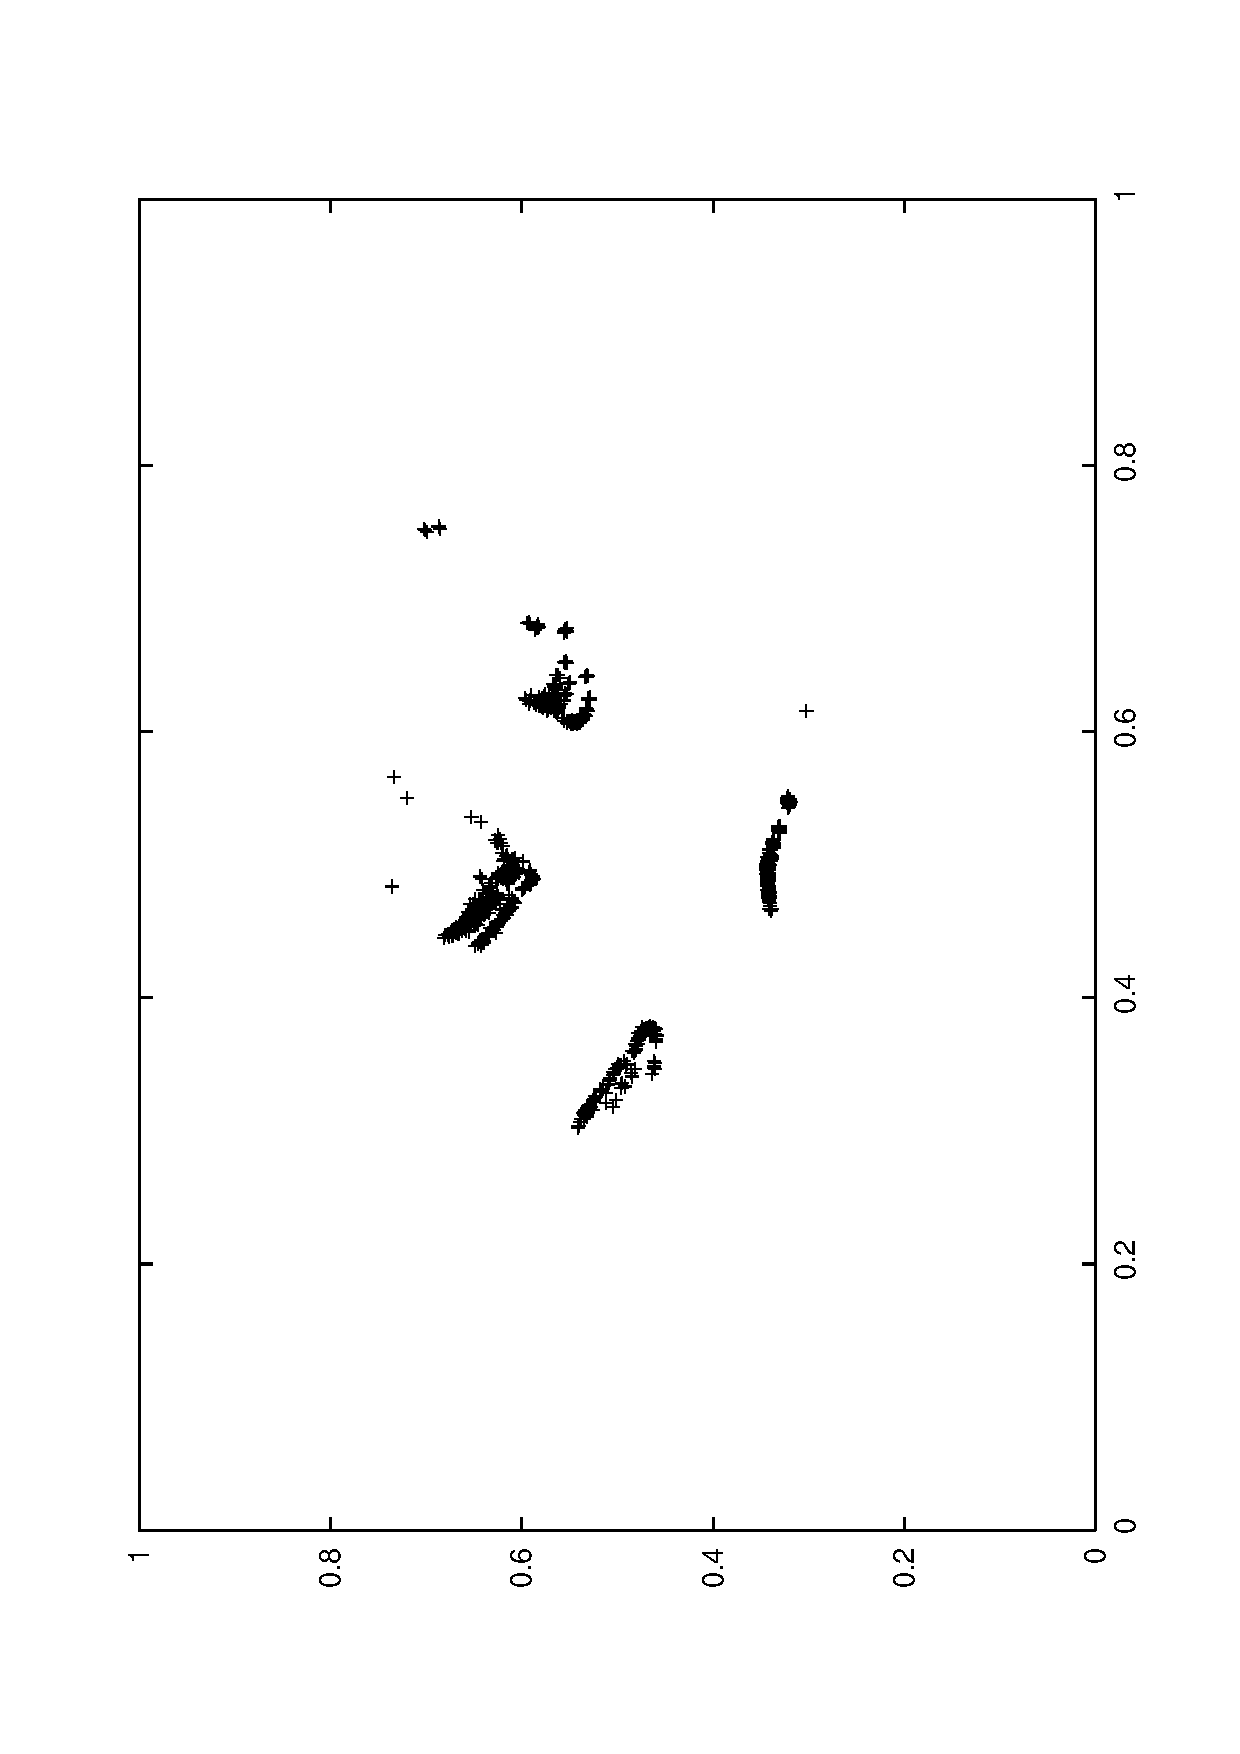
\includegraphics[angle=270, width=0.48\textwidth]{\pth/crim1}
\ 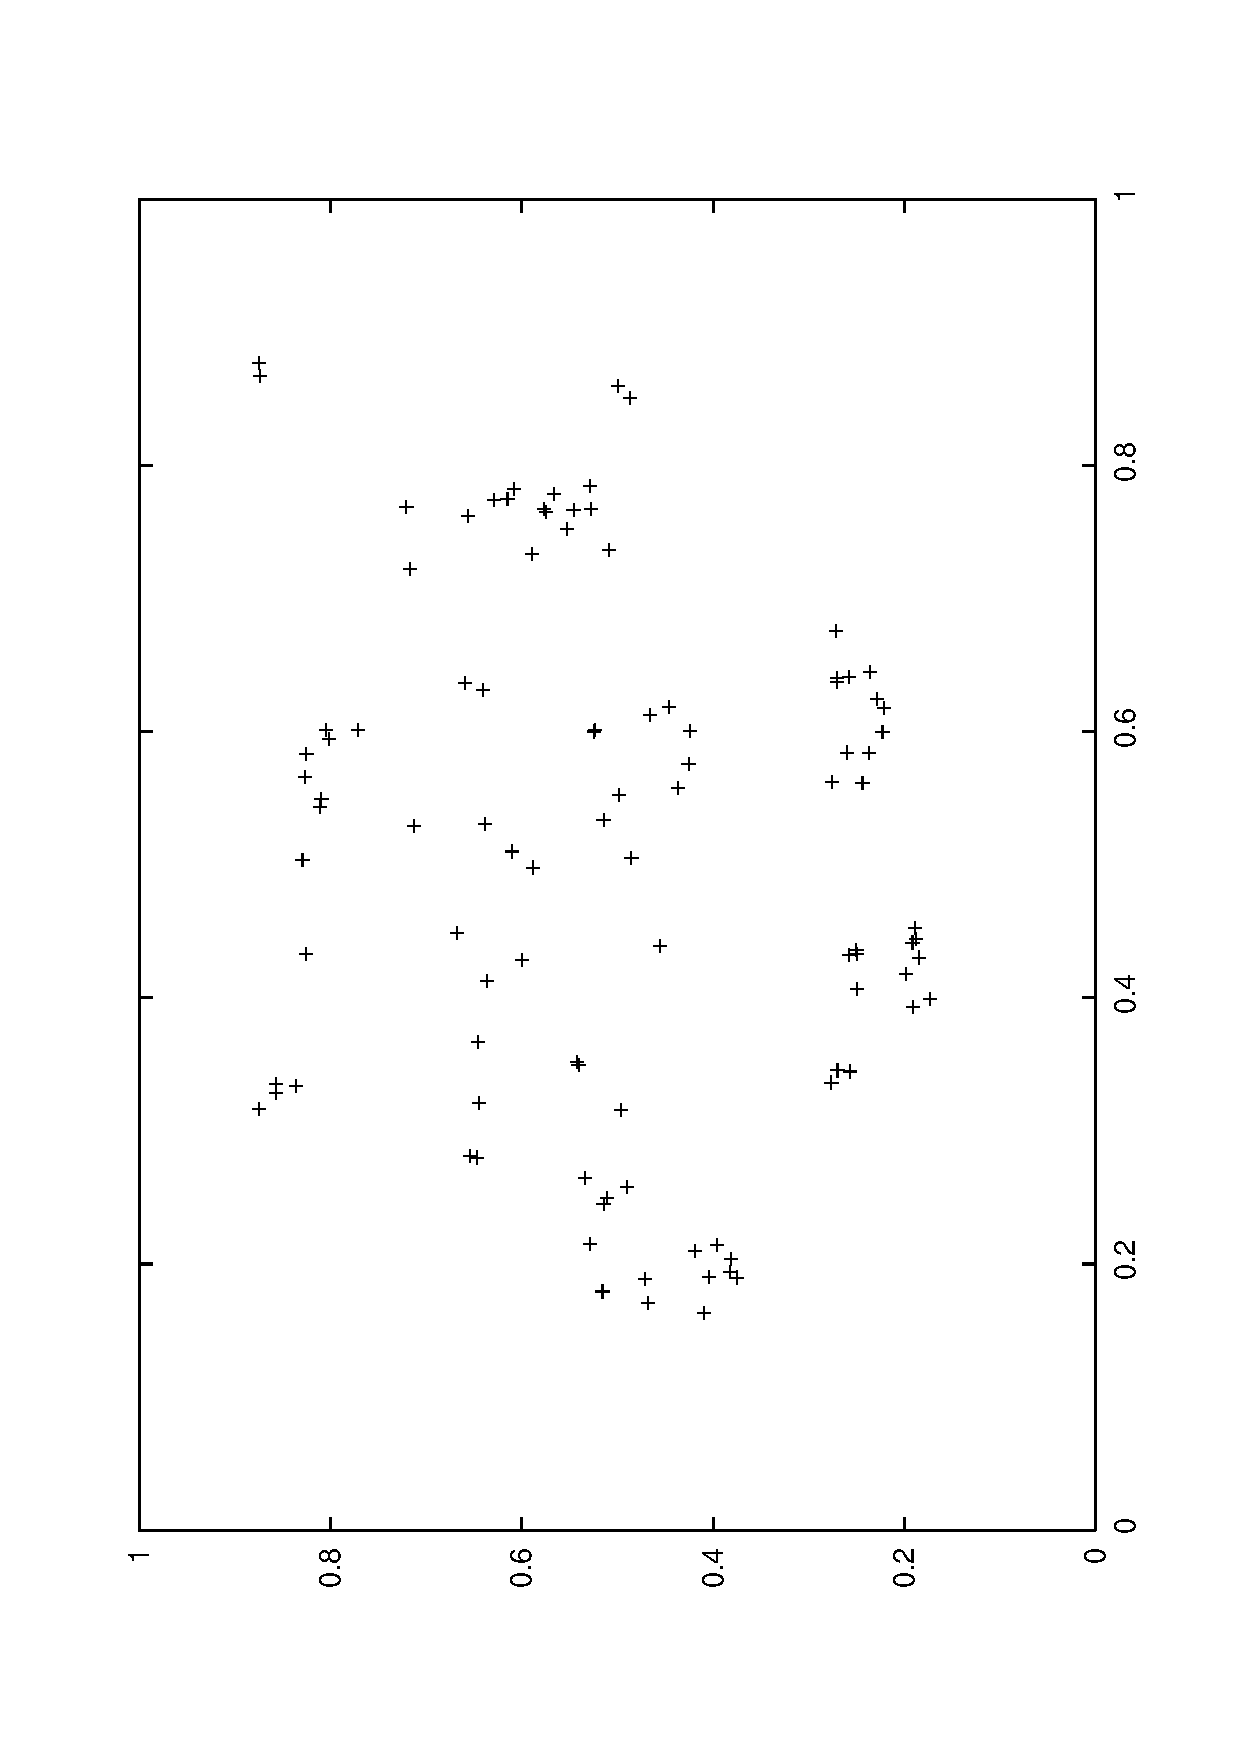
\includegraphics[angle=270, width=0.48\textwidth]{\pth/crim2}
\caption{Visualisation of criminals, non flat case.
Left: with categories; right: without categories.}
\label{to:fig:cluscrimcat}
\end{center}
\end{figure}

In Figure~\ref{to:fig:cluscrimcat}, left, we see a visualisation of real data. We
have taken a database of $1,\!000$ criminal records \thesis{supplied to us by
the Dutch national police,} and divided the crimes into three categories
(light, middle, heavy): each record has three integers, describing the number
of crimes in the respective categories. The distance measure we use is one
defined on multisets and is described 
in\paper{~\cite{MMM}}\thesis{ Chapter~\ref{ch:MMM}}. It basically averages the
absolute differences between the numbers of crimes.

The resulting matrix cannot be embedded in the plane, but it almost could,
since the mean error is relatively small $0.00494$ and so is the standard
deviation $0.00529$. We refer to this type of situation as a ``non flat
case''. An indication that the data is almost flat, is that the clustering
stays within the $0.5 \times 0.5$ sub-square, and inflation increases the
error. There are four main clusters in this picture, where:
\begin{itemize}
\item The leftmost one consists of criminals that have committed relatively
      light crimes. They all fall into the categories light and middle.
\item The top one consists of all-rounders, they have all committed crimes
      in all categories.
\item The rightmost one consists of criminals that have only committed
      light and heavy crimes, nothing in between.
\item The bottom one consists of criminals that have only committed light
      crimes, all of them fall into the category light.
\end{itemize}
Then there is a very small cluster in the top-right corner of the picture, this
is a cluster of people who have only committed heavy crimes. This is apparently
non-standard behaviour for a criminal. There are a few other isolated points in
this picture, they all are people with a strange criminal record.

In Figure~\ref{to:fig:cluscrimcat}, right, we see the clustering of $100$
criminals based upon the same distance measure as in
Figure~\ref{to:fig:cluscrimcat}, but now we do \emph{not} categorize the crimes;
here the records have 80 attributes. The result is a scattered image (largely
due to the lack of similarity), occupying a large part of the unit square, and
only a few local clusters. We make use of inflation factor $\sigma=2$ and
correction multiplier $\rho=1/16$ here, to produce the picture with a mean
error of $0.02636$ and a standard deviation of $0.01786$. All visualisations
are obtained within a few seconds.

Finally, we show an example from chemistry. The dataset we use, the so-called
$\mathtt{4069.no\_aro}$ dataset, contains 4,069 molecules (graphs); from this
we extracted a lattice containing the 2,149 most frequent subgraphs. These are
grouped into 298 structural related patterns occurring in the same molecules
using methods presented in~\cite{AIAI}, resulting in a 298 by 298 distance
matrix; the distance between graphs is based on the number of co-occurrences.

\begin{figure}[!ht]
\begin{center}
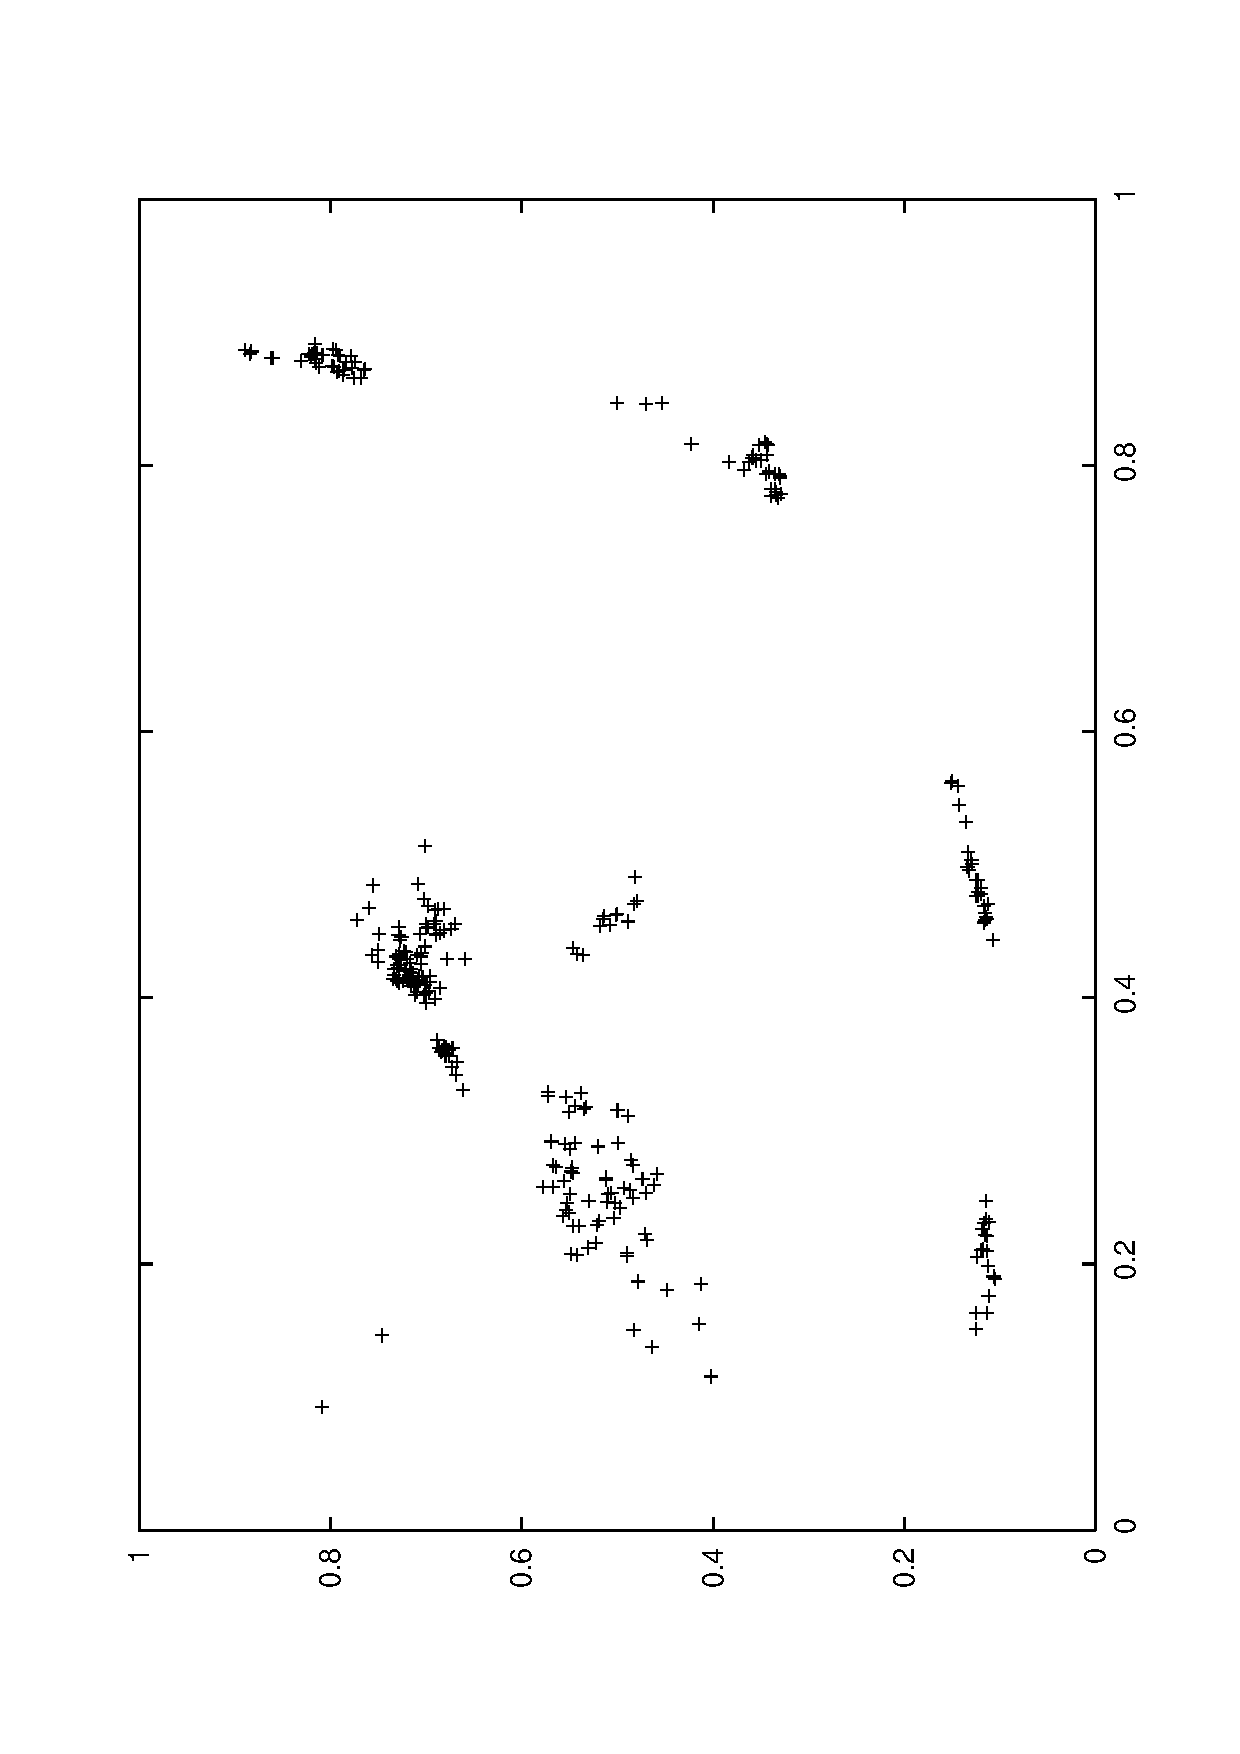
\includegraphics[angle=270, width=0.48\textwidth]{\pth/ed1}
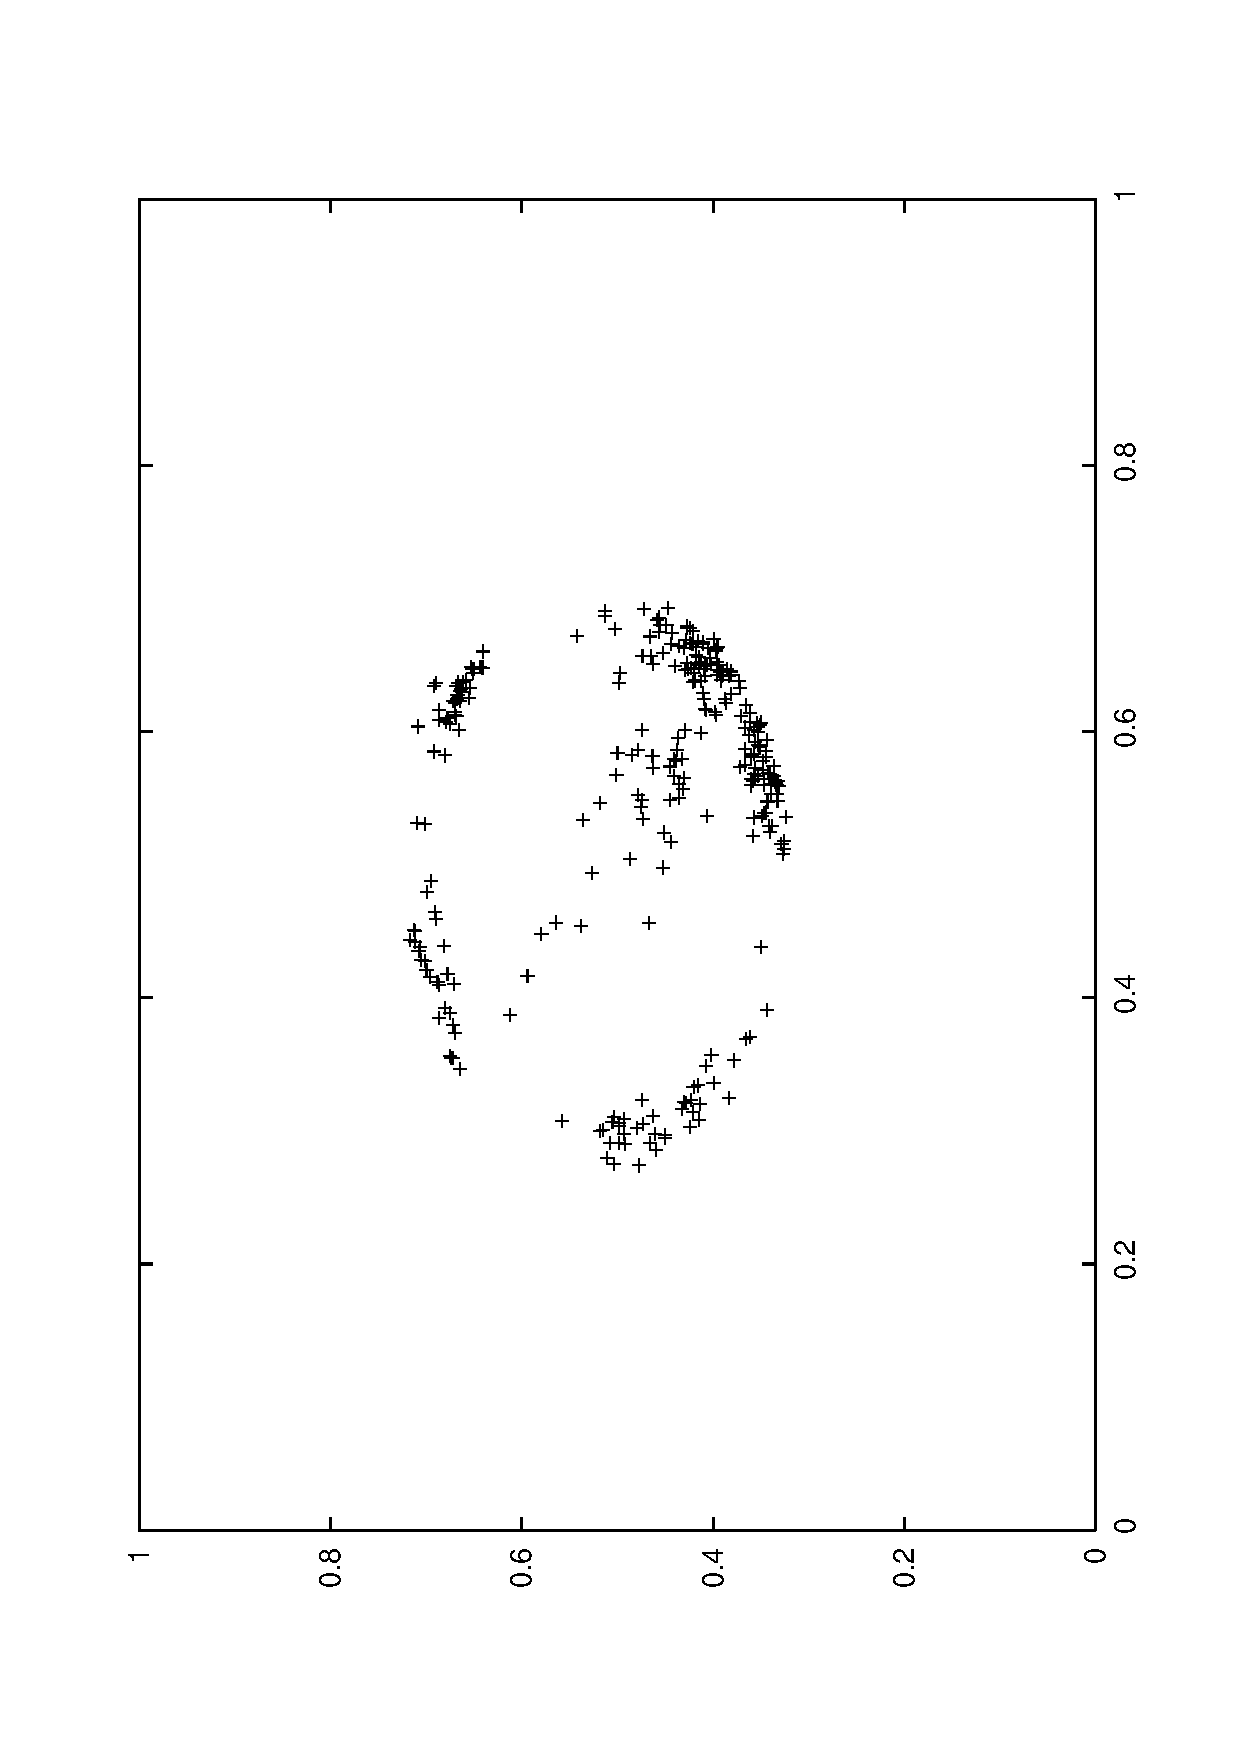
\includegraphics[angle=270, width=0.48\textwidth]{\pth/ed2}
\caption{Two visualisation of a dataset with molecules.} \label{to:fig:clused}
\end{center}
\end{figure}

Figure~\ref{to:fig:clused} shows two visualisations. The left-hand picture has
mean $0.03488$ and standard deviation $0.03117$, with parameters $\rho = 0.048$
and $\sigma = 1.1$; the right-hand picture has mean $0.05029$ and standard
deviation $0.03200$, with parameters $\rho = 0.031$ and $\sigma = 0.5$. The
latter picture is what we would have gotten when we had used a bounded unit
square. The first picture gives a better embedding, with a lower error. The
groups that pop up can be used by a biologist to investigate biological
activity.

\section{Conclusions and further research}\label{to:conclusion}
We conclude that our algorithm is able of giving adequate visualisations on the
torus. Starting from a set of data points and their pairwise distances, it
quickly provides an embedding on this surface. The algorithm is fast, flexible
and easy to use, for instance for clustering purposes.

The method was originally developed for the analysis of criminal records (see
Section~\ref{to:exps}), and performs quite well in this case, but it also appears
to be applicable in other fields.

For further research, we would like to examine other topologies, such as a
sphere. Yet another possibility is to somehow fix current points, once they
have reached a good position with respect to \emph{many} other points. And
finally, the online addition of new points.

\paper{
\section*{Acknowledgements}
This research is part of the DALE (Data Assistance for Law Enforcement) project
as financed in the ToKeN program from the Netherlands Organization for
Scientific Research (NWO) under grant number 634.000.430.\\ The authors would
like to thank Timo Krul for an insightful simplification of the distance
algorithm.

\bibliography{$HOME/projects/bibliography}{}
\bibliographystyle{plain}

\end{document}
}
